\documentclass[9pt,table]{beamer}
\usepackage{verbatim} % For using /begin{comment}; /end{comment}
\usepackage{graphicx}
\usepackage{helvet}
\usepackage{ragged2e}

% Tables
\usepackage{booktabs} % ??
\usepackage{multirow} % text in one cell can span multiple rows

\usepackage{textpos} % absolute positioning of text

% Put slide numbers at bottom right corner
\setbeamertemplate{footline}{%
    \raisebox{5pt}{\makebox[\paperwidth]{\hfill\makebox[10pt]{%
    \scriptsize\insertframenumber}}}}
\setbeamercolor{footline}{fg=gray}

\setbeamertemplate{navigation symbols}{}% Empty to get rid of them!
%\useoutertheme{infolines}

%\addtobeamertemplate{block begin}{\vspace{-8pt}}{}
\setbeamerfont{frametitle}{series=\bfseries}

\setbeamertemplate{itemize items}{$\bullet$}
%\setbeamertemplate{itemize items}{$\circ$}
%\setbeamertemplate{itemize items}[circle]

\setbeamercolor{background canvas}{bg=white}
\setbeamercolor{normal text}{fg=black}
\setbeamercolor{title}{fg=black}
\setbeamercolor{frametitle}{fg=black}
\setbeamercolor{framesubtitle}{fg=black}
\setbeamercolor{block title}{fg=black}
\setbeamercolor{itemize item}{fg=black}
\setbeamercolor{itemize subitem}{fg=black}
\setbeamercolor{enumerate item}{fg=black}
\setbeamercolor{enumerate subitem}{fg=black}

%% Command for extra space for graphics... or something
\newcommand\Wider[2][3em]{%
    \makebox[\linewidth][c]{%
       \begin{minipage}{\dimexpr\textwidth+#1\relax}
           \raggedright#2
       \end{minipage}}}

%% Outline
\AtBeginSection[]{
    \begin{frame}<beamer>
        \frametitle{Outline}
        \tableofcontents[currentsection]
    \end{frame}}

%% Title slide
\title{\textbf{Determining the size of Coronal Bright Points using cross-correlation
    methods and data from AIA/\textit{SDO}}}
%\subtitle{\textbf{ASTR 598}}
\author{\textbf{Laurel Farris}}
\date{10 April 2017}
  
\begin{document}
%{\usebackgroundtemplate{\includegraphics[width=\paperwidth]
%    {awesome.jpg}}
%\begin{frame}
%    \titlepage{}
%\end{frame}}

%\begin{frame}{Magnetohydrodynamics (MHD)}{Theory}
%    \begin{block}{Equations of ideal MHD}
%        \begin{list}{}
%            \item \textcolor{tan}{mass continuity equation}
%                $\frac{\partial\rho}{\partial{t}} +
%                \nabla\left(\rho\mathbf{V}\right) = 0 $
%            \item \textcolor{tan}{equation of motion}
%                $\rho\frac{\textrm{d}\mathbf{V}}{\textrm{d}t} =
%                -\nabla{P} - \frac{1}{\mu_{0}}\mathbf{B}\times\left(
%                \nabla\times\mathbf{B}\right) $
%            \item \textcolor{tan}{energy equation}
%                $\frac{\textrm{d}}{\textrm{d}t}
%                \left(\frac{P}{\rho^{\gamma}}\right) = 0$
%            \item \textcolor{tan}{induction equation}
%                $\frac{\partial\mathbf{B}}{\partial{t}} =
%                \nabla\times\left(\mathbf{V}\times
%                \mathbf{B}\right)$
%        \end{list}
%    \end{block}
%    Add more about just theory here.
%\end{frame}

%{\usebackgroundtemplate{\includegraphics[height=\paperheight]
%    {loop.jpg}}
%\begin{frame}
%\end{frame}}

\begin{frame}
    \titlepage{}
\end{frame}

\begin{frame}{Outline}
    \tableofcontents
\end{frame}

\section{Introduction}

\begin{frame}{What is a Coronal Bright Point (CBP)?}{General}
    \begin{itemize}
        \item Aka. X-ray bright point
        \item Ubiquitous across solar disk
        \item Dominate during solar minimum
        \item Emerging flux vs. cancelling bipoles
            (opposite polarity magnetic features cancelling)
        \item Lifetimes: 1 hour - $\sim$ few days
        \item Size $\sim$ 10-30 arcsec (22 Mm); cores $\sim$4-7 Mm
    \end{itemize}
    \begin{center}
        \begin{tabular}{c|c|c|c|}
            \cline{2-4} & {\textbf{\textcolor{red}{period}}} &
            {\textbf{\textcolor{red}{decay time}}} &
            {\textbf{\textcolor{red}{velocity}}}\\
            \hline \multicolumn{0}{|c|}{\textcolor{blue}{kink osc}} &
                2{-}20 m & quickly & ---\\
            \hline \multicolumn{0}{|c|}{\textcolor{blue}{sausage osc}} &
                30 s -- 7 m & --- & ---\\
            \hline \multicolumn{0}{|c|}{\textcolor{blue}{acoustic osc}} &
                7{-}31 m & 5{-}30 m & 200 km s$^{-1}$\\
            \hline \multicolumn{0}{|c|}{\textcolor{blue}{acoustic waves}} &
            140{-}420 s (2{-}7 m) & --- & 35{-}165 km s$^{-1}$\\
            \hline \multicolumn{0}{|c|}{\textcolor{blue}{fast waves}} &
                --- & --- & $>$150 km s$^{-1}$\\
            \hline \multicolumn{0}{|c|}{\textcolor{blue}{torsional modes}} &
                10 m & long & 1000 km s$^{-1}$\\
            \hline
        \end{tabular}
    \end{center}
    Highlight size here, lead-in to cross-correlations.
\end{frame}

\begin{frame}{}
    %\includegraphics{full_disk}
\end{frame}

\section{Maths}
\begin{frame}[t, label=main]{Cross-correlation}
    \[
        f(t) \star g(t) = f(-t) \ast g(t)
        \]
    \begin{columns}[t]
        \column{0.5\textwidth}
        Here is some text.
        \column{0.5\textwidth}
        Put some simple curves here to illustrate cc=1, -1, etc.
        Then show two lightcurves from actual data set.
    \end{columns}
    \hyperlink{supplemental}{\beamerbutton{here}}
\end{frame}
\appendix
\section{More}
\begin{frame}[label=supplemental]
    Supplemental content.

    Back to \hyperlink{main}{\beamerbutton{main}}
\end{frame}
\begin{frame}
    \begin{block}{Block title}
        Text.
    \end{block}
    \begin{block}
        Text.
    \end{block}
\end{frame}

%{%
%\setbeamercolor{background canvas}{bg=black}
%\setbeamertemplate{background}{%
%\parbox[c][\paperheight][c]{\paperwidth}{%
%%\hspace{3cm}
%\centering
%\includegraphics[height=\paperheight]{figures/full_disk.png}}}
%\begin{frame}[t]{Research}{AIA/\emph{SDO}}
%    \hspace{-2em}Fe {\footnotesize XII, XXIV}\\
%    \hspace{-2em}193 \AA{}\\
%\end{frame}}
%
%\begin{frame}{Research}{Cross-correlations}
%    \begin{block}{}
%        Text.
%    \end{block}
%    \begin{block}{}
%    \Wider[4em]{%
%    \begin{center}
%        \includegraphics[width=\textwidth]{test2.png}
%    \end{center}}
%    \end{block}
%\end{frame}


\end{document}
